%-------------------------------------------------------------
% Language
% Use the option "language=EN" to set the beamer theme in English. Use
% the option "language=ES" to set the beamer theme in Spanish.

% Colors
% Use the option "color=white" to set the background in white and the
% bottom bar in blue. Use the option "color=blue" to set the
% background in blue and the bottom bar in white. Use the option
% "color=blue2" to set the background in blue and the bottom bar in
% blue.

% Font Color
% Use the option "fontc=black" to set the font color in black. If this
% argument is not given the default color is set depending of the
% color scheme selected.

% Credits: https://github.com/alejogm0520 & Samuel Plazas Escudero
%-------------------------------------------------------------

%--Principal packages
\documentclass[aspectratio=43,8pt]{beamer} % 4:3, can be 16:9
\usetheme[language=EN, color=white]{EAFIT}
\usepackage[english]{babel}
%\decimalpoint % All decimal numbers with point
\usepackage[utf8]{inputenc}
\selectlanguage{english}
\usepackage{amsmath,amsfonts,amssymb,cancel,physics} % Equations
\usepackage{verbatim} % Environments, \begin{comment}
%--Arial
\usepackage{helvet}
\renewcommand{\familydefault}{\sfdefault}
%--Beamer packages
\usepackage{tikz} % For making vectorized figures, arrows
\usepackage{ifthen} % For specifying conditionals for sections
\usepackage{ragged2e}\justifying % Whole text justified, except enumerate: add \justifying
\usepackage{xcolor}
\usepackage{multicol} % Multiple columns in one frame
%--Tables-Figures
%\renewcommand\spanishtablename{Tabla}
\usepackage{booktabs,multirow} % Bookstyle tables
%-Figure label
\usepackage[labelsep=period,justification=justified,format=plain]{caption} % Dot instead of colon and justified caption
%--Figure
\usepackage{graphicx,subcaption} % Figures and subfigures
\graphicspath{{Media/}} % Media rute
%-Figure-Table on top
\usepackage{float} % Allows to put H instead of ht
\setbeamertemplate{caption}[numbered] % Numbered captions
%---------TOC
\setbeamertemplate{section in toc}[sections numbered]
\setbeamertemplate{subsection in toc}[subsections numbered]
\setbeamerfont{section in toc}{size=\small}
\setbeamerfont{subsection in toc}{size=\footnotesize}
\setbeamertemplate{subsection in toc}{\leavevmode\leftskip=3.2em\rlap{\hskip-2em\inserttocsectionnumber.\inserttocsubsectionnumber}\inserttocsubsection\par} % Indented subsection
\setcounter{secnumdepth}{0}
%---------Cite
\usepackage{bibentry} % Full cite foot
%\nobibliography* % Full cite foot
% Or: \setbeamertemplate{bibliography item}[]% [online][book][article][triangle][text]
\setbeamertemplate{bibliography item}{\insertbiblabel} 
\usepackage{etoolbox} % Package for using justified bibliography 
\apptocmd{\thebibliography}{\justifying}{}{} % Justified bibliography 
%---------Footnotes
\setbeamercolor{footnote}{fg=white}
\setbeamercolor{footnote mark}{fg=.} % Takes the color depending on the circumpstance
\setbeamercolor{bibliography entry author}{fg=white} % Allows to have white footnote bibs
\setbeamertemplate{footnote}
{
  \hspace*{-1cm} % Horizontal movement
  \vspace*{-2.88cm} % Vertical movement
  \parbox[c][3.4cm]{10.6cm}{\tiny\noindent\insertfootnotemark\insertfootnotetext} % b: bottom, height: 3.3cm, horizontal length: 10.6cm (max horizontal)
% If there are problems, put -2.87cm and 3.3cm
}
\renewcommand{\footnoterule}{\kern -3pt \hrule width \textwidth height 0pt\kern 3pt} % No footnoterule
%------------------------------------
%---------Numbered Slides and Sections
\setbox0=\hbox{\subsecname\unskip}\ifdim\wd0=0pt\else%
 ~--~\insertsubsectionhead
\fi
%------Numbering section: title in bold, centered and with a line
\newcommand{\numb} 
{
  \setbeamertemplate{frametitle}
  {
    \ifx\insertsubsection\empty % No subsection
         \bfseries\thesection.~\insertframetitle~\color{black}\par\vskip-5pt\hrulefill % \centering
    \else % subsection
         \bfseries\thesection.~\insertframetitle~\color{black}\par\vskip-9pt\hrulefill\par\vskip3pt{\large\thesection.\thesubsection~\insertframesubtitle} % Subsection with smaller size;
    \fi
  }
}
%------No numbering section: title in bold, centered and with a line
\newcommand{\nonumb}
{
  \setbeamertemplate{frametitle}{\bfseries\color{black}\centering\insertframetitle\par\vskip-6pt\hrulefill}
}
%------------------------------------
%--No hyphenation on text
\tolerance=1
\emergencystretch=\maxdimen
\hyphenpenalty=10000
\hbadness=10000
%------------------------
%---------Itemize justified in beamer
\makeatletter
\renewcommand{\itemize}[1][]{
  \beamer@ifempty{#1}{}{\def\beamer@defaultospec{#1}}
  \ifnum \@itemdepth >2\relax\@toodeep\else
    \advance\@itemdepth\@ne
    \beamer@computepref\@itemdepth % Sets \beameritemnestingprefix
    \usebeamerfont{itemize/enumerate \beameritemnestingprefix body}
    \usebeamercolor[fg]{itemize/enumerate \beameritemnestingprefix body}
    \usebeamertemplate{itemize/enumerate \beameritemnestingprefix body begin}
    \list
      {\usebeamertemplate{itemize \beameritemnestingprefix item}}
      {\def\makelabel##1{
          {
            \hss\llap{{
                \usebeamerfont*{itemize \beameritemnestingprefix item}
                \usebeamercolor[fg]{itemize \beameritemnestingprefix item}##1}}
          }
        }
      }
  \fi
  \beamer@cramped
  \justifying % Justified itemize
  \beamer@firstlineitemizeunskip
}
\makeatother
%------------------------
%---------get current section name for showing it at its begining
\usepackage{nameref}
\makeatletter
\newcommand*{\currentname}{\@currentlabelname}
\makeatother
%---------Shows in which section we are at the begining of each one
\AtBeginSection[]
{
\begin{frame}[plain,noframenumbering]
  \begin{beamercolorbox}[ht=\paperheight,wd=\paperwidth, center]{Portada}
    \begin{center}\textbf{\LARGE \currentname}\end{center} % Leave the next space mandatorily

    \vspace{0.44\paperheight}
  \end{beamercolorbox}
\end{frame}
}

%---------TEXTBLOCKS-GRID 
\usepackage[absolute,overlay,showboxes]{textpos}
%\usepackage[texcoord,grid,gridunit=mm,gridcolor=red!10,subgridcolor=green!10]{eso-pic} % Helping grids, comment when publishing
%---------COLOR DEFINITIONS
\definecolor{azure(colorwheel)}{rgb}{0.0, 0.5, 1.0} % Define colors here
\definecolor{miscblue}{RGB}{0,0,75}


%%%%%%%%%%%%%%%%%%%%%%%
%Start of the Document%
%%%%%%%%%%%%%%%%%%%%%%%

%---------COVER PAGE

\title{\textit{DATA STRUCTURE FOR EFFICIENT INDEXING OF\\[1ex] FILES AND DIRECTORIES}} 

\author{\normalfont\large\texorpdfstring{\textbf{\textcolor{miscblue}{\textit{Juan S. Cárdenas R.\\ David Plazas E.}}}}{}} % PI3


\def\carrera{Engineering Mathematics}
\def\departamento{Departament of systems and informatics }
\def\escuela{School of science}
\def\eafit{\textit{\textcolor{miscblue}{Universidad EAFIT}}}
\def\materia{Data structures and algorithms I}
%\def\materia{Proyecto Avanzado I}
\def\fecha{\textit{\textcolor{miscblue}{2017}}}
\def\city{\textit{\textcolor{miscblue}{Medellín}}}
% to add more def, search for "Dirección" in beamerthemeEAFIT.sty



%\includeonly{c/ex}
\begin{document}

\nonumb % Not numbered titles
\begin{frame}
% Portada Inspira Crea Transforma
\end{frame}
%%%%%%%%%%%%%%%%%%%%%%%%%%%%%%%%%%%%%%%%%%%%%%%%%%%%%%%%%%%%%%%%%%%%%%%%%%%%
\begin{frame}
\begin{center}
  \titlepage % Cover page
\end{center}
\end{frame}



\numb % Numbered titles
%\include{ex_beamer} % Comment when publishing
\section{Designed Data Structure}
\begin{frame}{Designed Data Structure: NashTable}
	\begin{figure}[H]
  		\centering
  		\includegraphics[scale = 0.4]{NashTable}
  		\caption{Example of a NashTable. Each Nash has a hash table of Branch objects. Each Branch object has another Nash and a LinkedList of dictionaries. Files are indexed according to each character of their names.}
	\end{figure}
\end{frame}
\section{Data Structure Operations}
\subsection{Insertion}
\begin{frame}{Data Structure Operations}
\framesubtitle{Insertion \boldmath{$O(n)$}}
\begin{figure}[H]
  \centering
  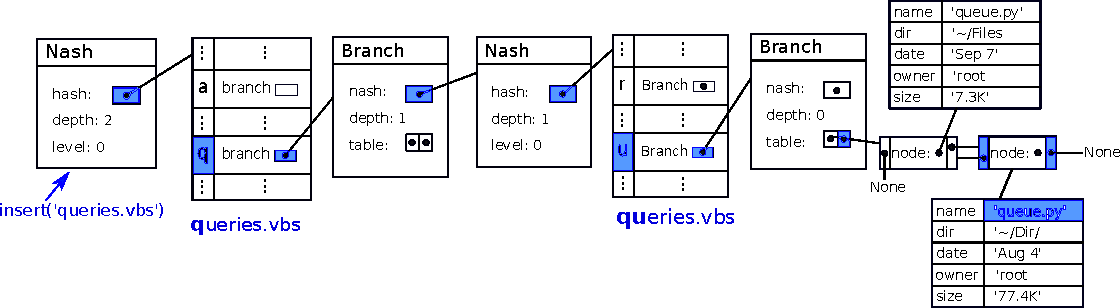
\includegraphics[scale = 0.6]{NashInsert.pdf}
  \caption{Insertion in NashTables.}
\end{figure}
\end{frame}
%%%%%%%%%%%%%%%%%%%%%%%%%%%%%%%%%%%%%%%%%%%%%%%%%%%%%%%%%
\subsection{Deletion}
\begin{frame}{Data Structure Operations}
\framesubtitle{Deletion \boldmath{$O(n)$}}
\begin{figure}[H]
  \centering
  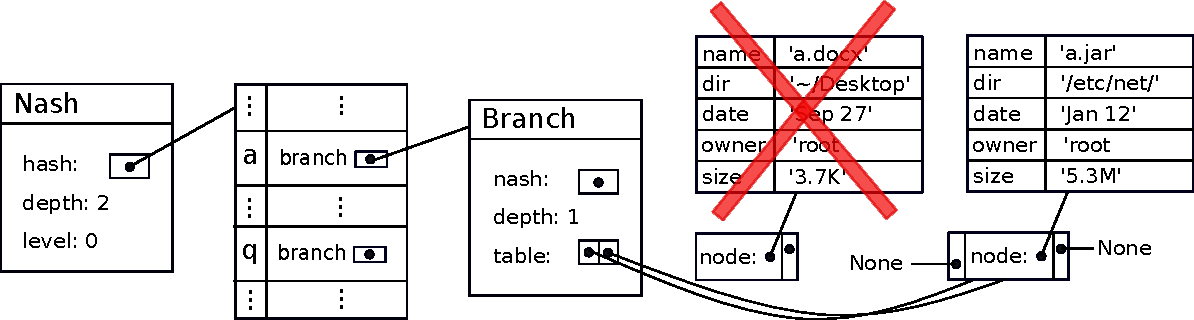
\includegraphics[scale = 0.55]{NashRemove.pdf}
  \caption{Deletion in NashTables.}
\end{figure}
\end{frame}
%%%%%%%%%%%%%%%%%%%%%%%%%%%%%%%%%%%%%%%%%%%%%%%%%%%%%%%%%
\subsection{Search}
\begin{frame}{Data Structure Operation}
\framesubtitle{Search \boldmath{$O(n+k)$}}
\begin{figure}[H]
  \centering
  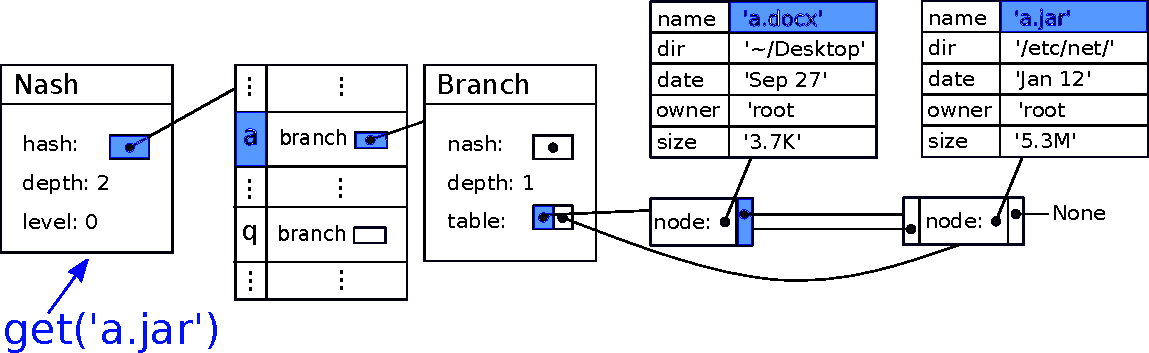
\includegraphics[scale = 0.55]{NashGet.pdf}
  \caption{Search in NashTables.}
\end{figure}
\end{frame}
\section{Design Criteria of the Data Structure}
\begin{frame}{Design Criteria of the Data Structure}
	\begin{itemize}
	\item The NashTable is based on hash tables and doubly linked lists; searching files is the priority.
    \item Although this first approach to solve the problem is not optimized for low memory consumption, it has been developed for optimize searching with different options.
    \item Hash tables were used since they are able to search for files in constant time.
    \item Double linked lists because insertion in the last position is achieved in constant time and also because they do not have a fixed size (unlike arrays), allowing the NashTable to add objects depending on the files indexed.
    \item Searching for files is independent from the amount of files indexed inside the structure. It just depends on the number of characters on the name.
	\end{itemize}
\end{frame}
\section{Time and Memory Consumption}
\begin{frame}{Time and Memory Consumption}
	
  \begin{table}
  \centering
  \caption{Execution time for each operation}
  \label{tab:exTime}
  \begin{tabular}{cccc}
  \hline
  \multirow{2}{*}{\textbf{Operation}} & \multicolumn{3}{c}{\textbf{Average Time}}                    \\ \cline{2-4} 
                                      & \textbf{DataSet 1} & \textbf{DataSet 2} & \textbf{DataSet 3} \\ \hline
  Create                              & $213.355ms$        & $5453.520ms$       & $29177.054ms$      \\
  Insert                              & $0.623ms$          & $0.046ms$          & $0.050ms$          \\
  Search                              & $0.026ms$          & $0.022ms$          & $0.023ms$          \\
  Remove                              & $0.018ms$          & $0.020ms$          & $0.020ms$          \\ \hline
  \end{tabular}
  \end{table}

  \begin{table}[h]
    \centering
    \caption{Memory consumption.}
    \label{table:mem}
    \begin{tabular}{cccc}
      \hline\rule{0pt}{2ex}
      \textbf{Memory Consumption} & \textbf{DataSet1} & \textbf{DataSet2} & \textbf{DataSet3} \\ \hline\rule{0pt}{2ex}
      Memory                     & 96.72MB & 475.136MB & 1638.4MB           \\ \hline
    \end{tabular}
  \end{table}
\end{frame}
\section{Implementation}
%%%%%%%%%%%%%%%%%%%%%%%%%%%%%%%%%%%%%%%
\begin{frame}{Implementation}
	\begin{figure}[H]
  		\centering
  		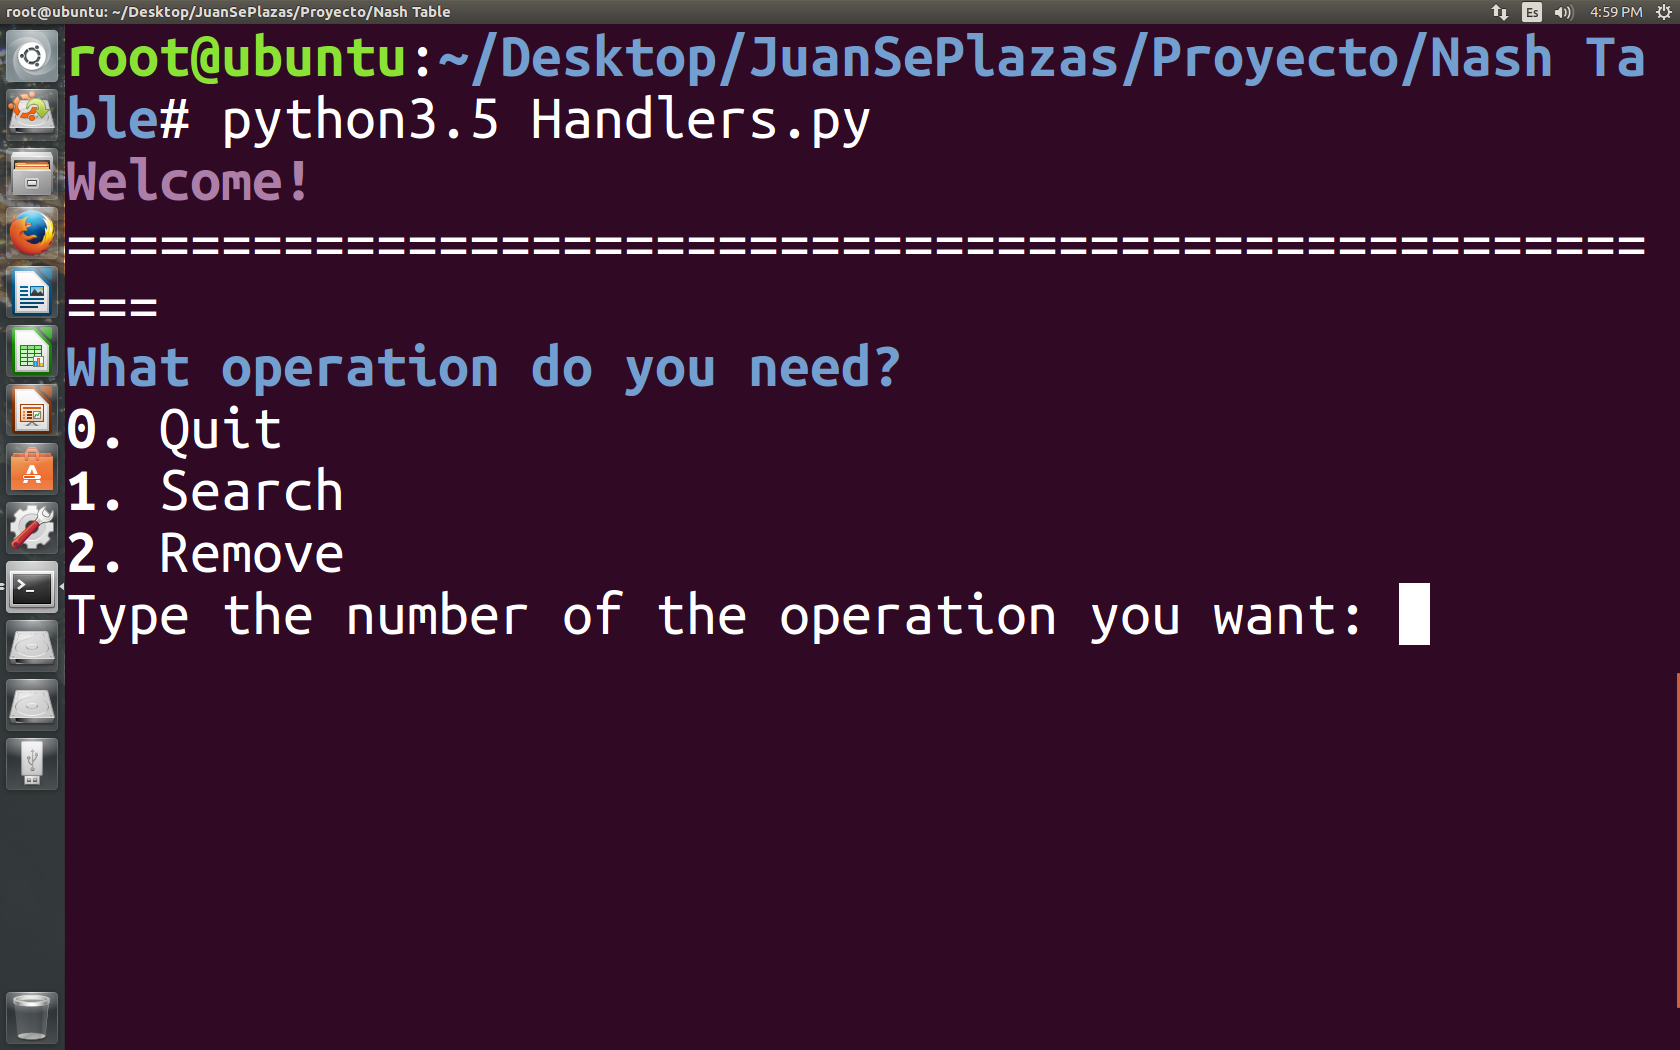
\includegraphics[scale = 0.1575]{GUI.png}
  		\caption{Example of GUI.}
	\end{figure}
\end{frame}
%%%%%%%%%%%%%%%%%%%%%%%%%%%%%%%%%%%%%%%
\begin{frame}{Implementation}
	\begin{figure}[H]
  		\centering
  		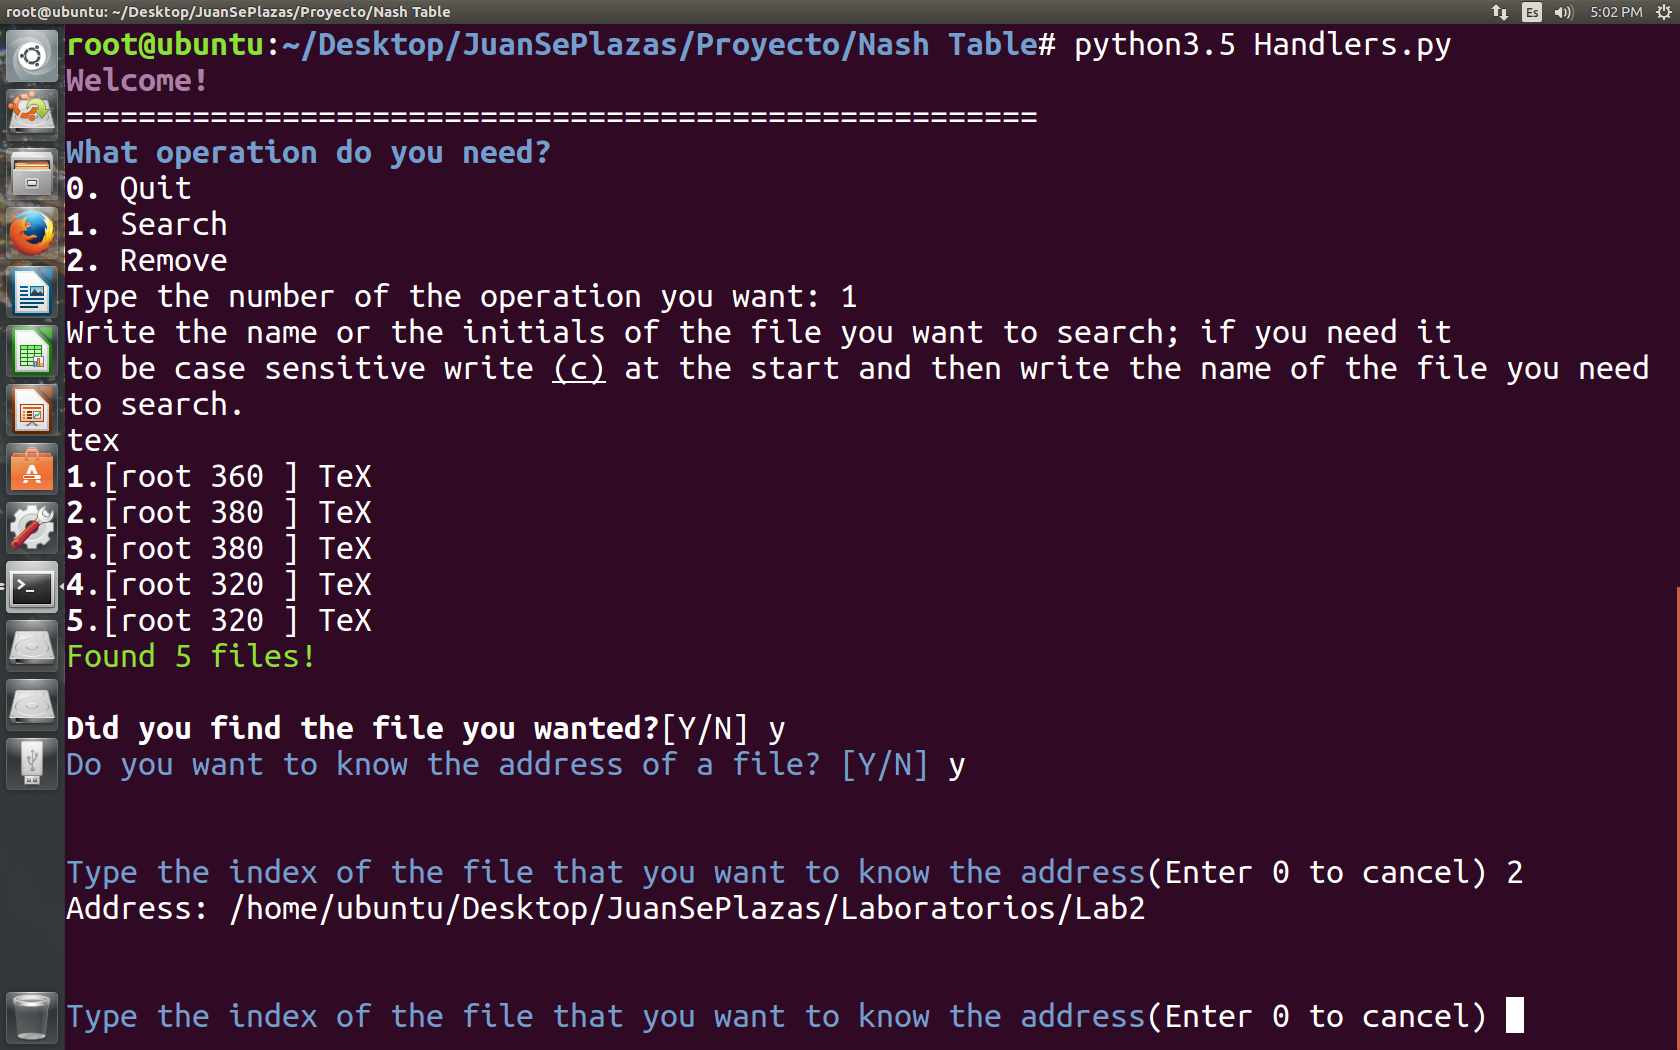
\includegraphics[scale = 0.1575]{ExampleSearch.png}
  		\caption{Example when searching for ``tex''.}
	\end{figure}
\end{frame}
%%%%%%%%%%%%%%%%%%%%%%%%%%%%%%%%%%%%%%%
\begin{frame}{Implementation}
	\begin{figure}[H]
  		\centering
  		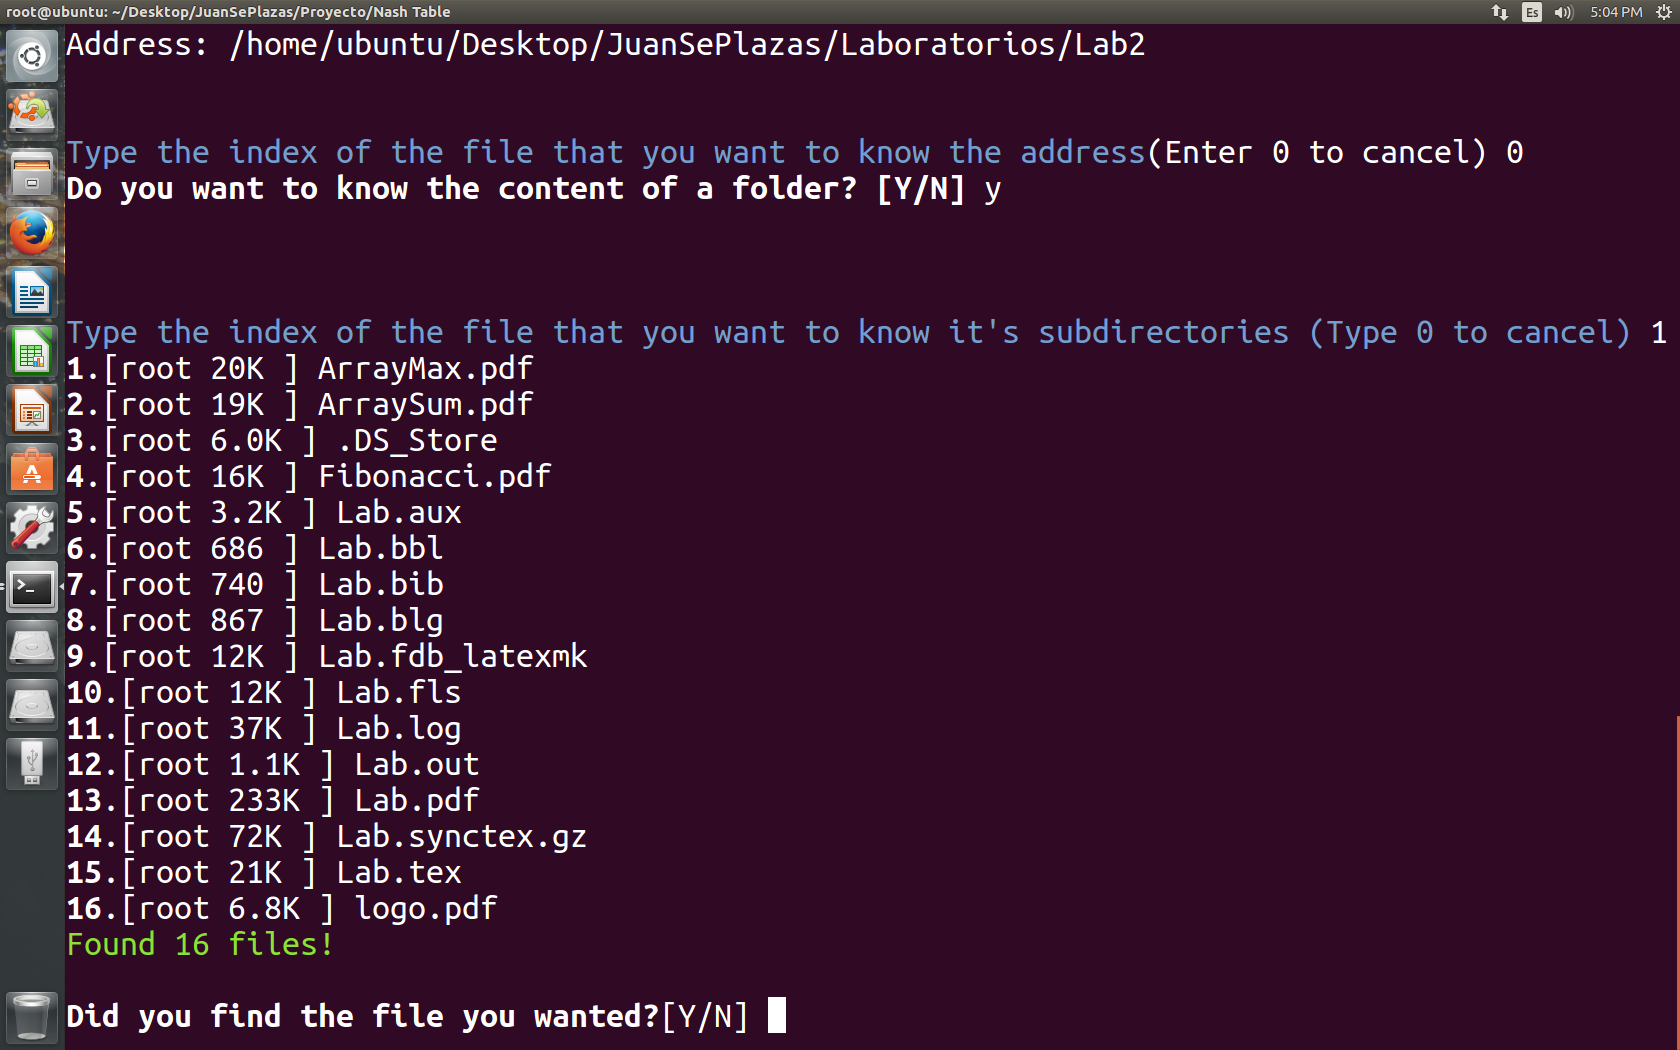
\includegraphics[scale = 0.1575]{ExampleSearchFolder.png}
  		\caption{Example when searching inside the first folder.}
	\end{figure}
\end{frame}
%%%%%%%%%%%%%%%%%%%%%%%%%%%%%%%%%%%%%%%
\begin{frame}{Implementation}
  \begin{figure}
      \centering
      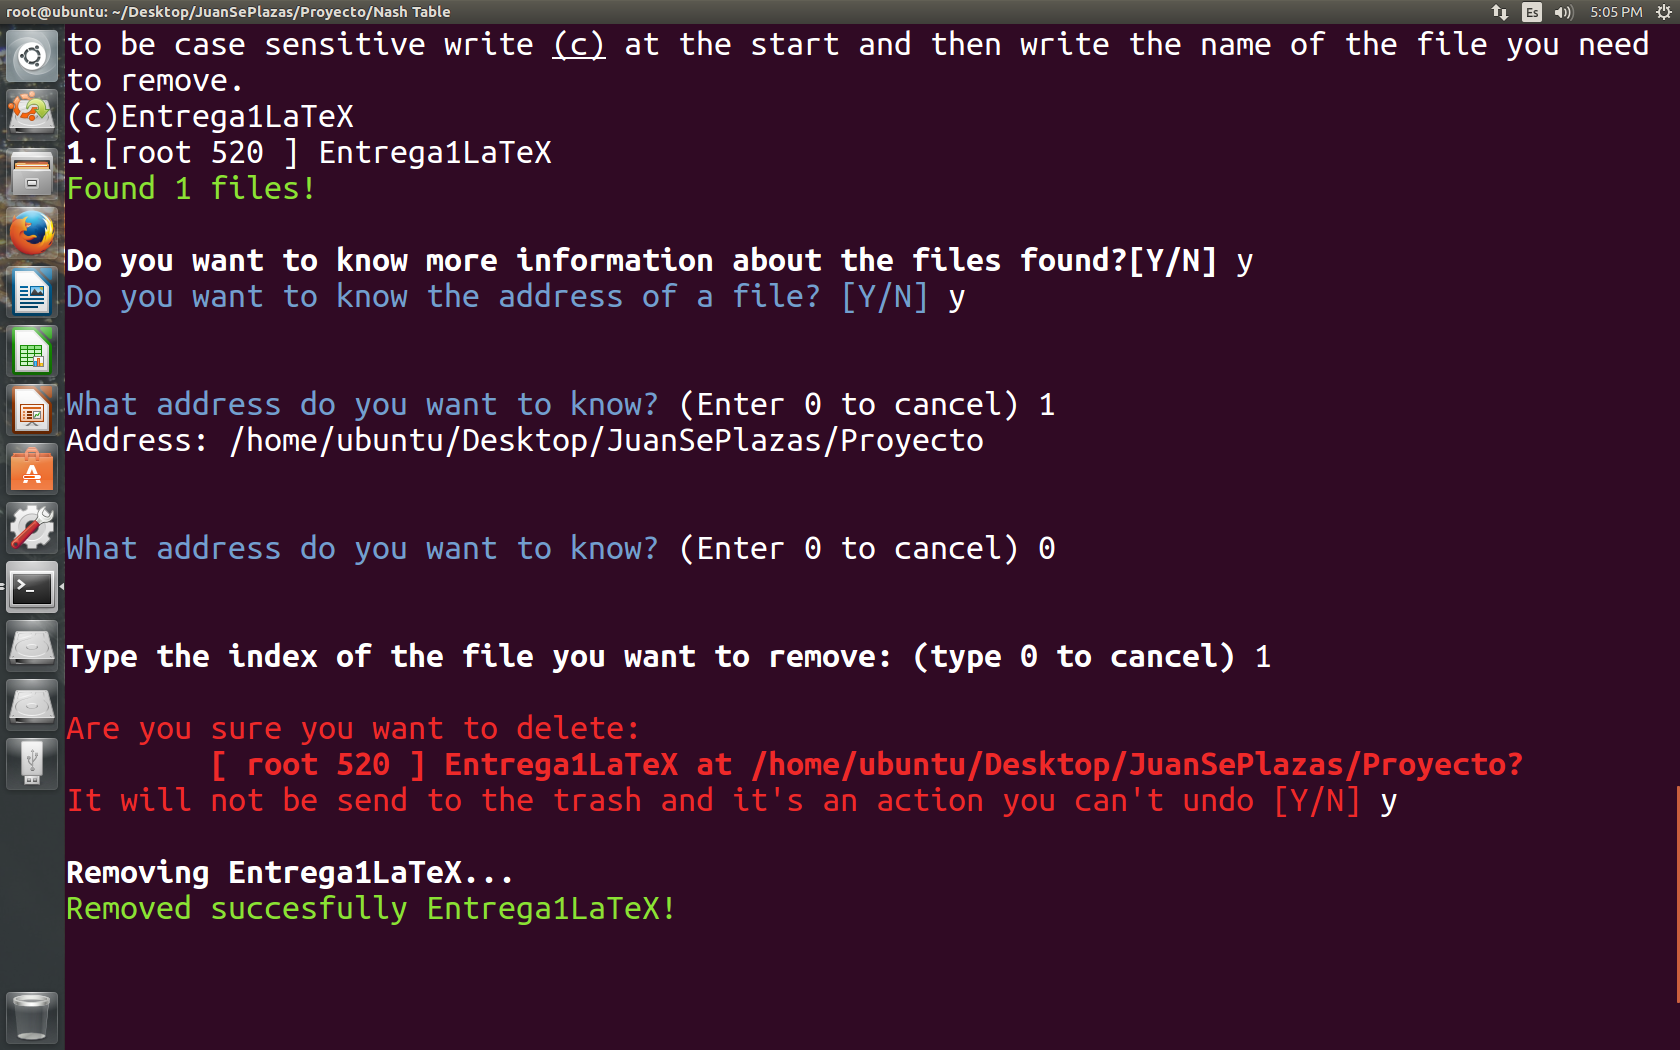
\includegraphics[scale = 0.1575]{ExampleRemove.png}
      \caption{Example of removal.}
  \end{figure}
\end{frame}
\nonumb % Not numbered titles
%\addcontentsline{toc}{section}{\small\protect\numberline{}{REFERENCIAS BIBLIOGRÁFICAS}} % Separated from other contents, for small number of contents
\addcontentsline{toc}{section}{\small REFERENCES} % Closer from other contents, for large number of contents
\nocite{*} % All citations showed (take care with fraud!)
%%%%%%%%%%%%%%%%%%%%%%%%%%%%%%%%%%%%%%%%%%%%%%%%%%%%%%%%%%%%%%%%%%%%%%%%%%%%
\section*{REFERENCES}
\begin{frame}[allowframebreaks]{REFERENCES} %  and put before {REFEREN...}
\begingroup % Group for changing the color
\renewcommand{\color}[1]{} % Allows to have black bibs and white footnote bibs
\small{\bibliographystyle{IEEEtran}} % Size of text; acm or gatech-thesis or ieeetr or ieeetran or icontec or iso690
\bibliography{ref}
\endgroup % Group for changing the color
% pdflatex -> bibtex -> pdflatex -> pdflatex
\end{frame}
%%%%%%%%%%%%%%%%%%%%%%%%%%%%%%%%%%%%%%%%%%%%%%%%%%%%%%%%%%%%%%%%%%%%%%%%%%%%
% Thank-slide
\begin{frame}[plain,noframenumbering] % No frame number
	\begin{beamercolorbox}[ht=\paperheight,wd=\paperwidth, center]{Portada}
		\begin{center}\Huge\textbf{Thank you}\end{center} % Or Thanks; leave the next space mandatorily
		
		\vspace{0.44\paperheight}
    \end{beamercolorbox}
\end{frame}
%%%%%%%%%%%%%%%%%%%%%%%%%%%%%%%%%%%%%%%%%%%%%%%%%%%%%%%%%%%%%%%%%%%%%%%%%%%%


\end{document}